
%(BEGIN_QUESTION)
% Copyright 2013, Tony R. Kuphaldt, released under the Creative Commons Attribution License (v 1.0)
% This means you may do almost anything with this work of mine, so long as you give me proper credit

Suppose you need to locate the anchor for a guy wire which will help support a power pole.  The 35 foot guy wire will attach to a point on the pole 26 feet above ground level:

$$\includegraphics[width=15.5cm]{i02682x01.eps}$$

Calculate the distance between the guy wire anchor and the base of the power pole ($x$), as well as the angle between the guy wire and the ground ($\theta$).

\vskip 10pt

$x$ = \underbar{\hskip 50pt} feet

\vskip 30pt

$\theta$ = \underbar{\hskip 50pt} degrees

\vskip 10pt


\underbar{file i02682}
%(END_QUESTION)





%(BEGIN_ANSWER)

$x$ = \underbar{23.43} feet

\vskip 30pt

$\theta$ = \underbar{47.98} degrees


%(END_ANSWER)





%(BEGIN_NOTES)


%INDEX% Mathematics review: trigonometric calculations

%(END_NOTES)


